%!TEX root = ./main.tex

\section{The Bipartite Setting}

% LEC 1

\subsection{Basic matching theory}

A well-known result characterizing bipartite graphs with perfect matchings is the following.

\begin{ftheo}[Hall's Theorem]
	A bipartite graph $G(X,Y)$ has a perfect matching iff $|X|=|Y|$ and $|\Gamma(S)| \ge |S|$ for all $S \subseteq X$.
\end{ftheo}

\begin{fcor}
	For $d \ge 1$, any $d$-regular bipartite graph has a perfect matching. In particular, it is decomposable into $d$ perfect matchings.
\end{fcor}

Henceforth, assume that $G$ is a bipartite graph with $|X|=|Y|\eqdef n$. Although it is easy through Hall's Theorem to figure out if $G$ \emph{has} a perfect matching, it is harder to count the number of perfect matchings. Indeed, counting turns out to be $\#\P$-hard, and even counting modulo a prime $p$ is hard. Any perfect matching of a bipartite graph may be thought of as a permutation $\sigma \in S_n$. Recall that any permutation $\pi$ has a sign
\[ \sign(\pi) = (-1)^{\text{number of even cycles in $\pi$}}. \]
See Section 1.1 of the author's Combinatorics I notes for more details.\\

We may associate with $G$ an $n \times n$ \emph{bipartite adjacency matrix} $M$, where $M_{ij} = 1$ iff the $i$th vertex in $X$ is adjacent to the $j$th vertex in $Y$. Note that
\[ \det(M) = \sum_{\sigma \in S_n} \sign(\sigma) \prod_{i=1}^n M_{i,\sigma(i)}. \]
Note that the product is nonzero (and in this case equal to $1$) iff $\sigma$ corresponds to a perfect matching of $G$. Consequently, if every perfect matching has the same sign, we can count the number of perfect matchings by merely looking at the absolute value of the determinant of the bipartite adjacency matrix. One interesting problem is to determine which graphs are such thata all perfect matchings have the same sign. We also have
\[ \perm(M) = \sum_{\sigma \in S_n} \prod_{i=1}^n M_{i,\sigma(i)} = \text{number of perfect matchings}, \]
but unlike the determinant, the permanent is hard to compute.\\

Let $M_1,M_2$ be perfect matchings of $G$. Note that $M_1 \triangle M_2$, the set comprising of the edges in precisely one of $M_1,M_2$, is a disjoint union of alternating cycles. Here, an alternating cycle means that the edges alternate being in $M_1,M_2$. $M_2$ has the same sign as $M_1$ iff there is an even number of cycles which have lengths divisible by $4$.\\
We can use the above observation to check if all matchings have the same sign. Given a perfect matching $M$, all permutations have the same sign (as $M$) iff there exists no cycle of length divisible by $4$ with edges alternating in $M$. How do we do this? First convert the bipartite graph to a directed one by assigning to each edge a direction from $X$ to $Y$. The problem then boils down to determining if there exists an even directed cycle in the graph obtained by contracting the matching edges. This seems simple, but is in fact far from trivial. We know now due to Seymour [cite] that this is possible in polynomial time. We do not discuss the details in general. \\
Consider the specific case where $G$ is $3$-regular. The Heawood graph is known to have all matchings of the same sign.
\begin{fex}[Heawood graph]
	The Heawood graph has vertex set $\Z_{14}$, 
\end{fex}
and we can use a construction procedure called the \emph{star product} (sometimes called \emph{splicing}) or to build up larger graphs with the same property. In fact, McCaig showed that the only $3$-regular graphs with this property are obtained in this manner from the Heawood graph. There is also only one strongly $2$-connected $2$-regular directed graph without any even cycle, which is obtained by contracting the Heawood graph. %\Z_7 with edge from x to x+1,x+3. can preserve similar to star product by u1 u2 u v1 v2 and u1' u2' u' v1' v2' by u1 u2 w v1' v2' and u1' v1 and u2' v2.

% LEC 2

\subsection{Pfaffians}

Now, requiring that all matchings have the same sign is rather restrictive. A better idea might be to change the non-zero entries of the bipartite adjacency matrix in a way that ensures nonzeroness of the overall determinant iff there exists a perfect matching. More specifically, Polya asked if we can we change some of the $1$ entries to $-1$ such that the resulting determinant becomes equal to the number of perfect matchings. For example, changing the bipartite adjacency matrix of $K_{2,2}$ to
\[ \begin{pmatrix} 1 & -1 \\ 1 & 1 \end{pmatrix} \]
makes the determinant equal to $2$, the number of perfect matchings. Another example is changing the bipartite adjacency matrix of $K_{3,3}$ with an edge removed to
\[ \begin{pmatrix} -1 & 1 & 1 \\ 1 & -1 & 1 \\ 1 & 1 & 0 \end{pmatrix}. \]
That is, Polya's problem asks whether some of the $1$s can be changed to $-1$s such that for any matching $\sigma$, $\sign(\sigma) = \prod_{i=1}^{n} a_{i\sigma(i)}$ (or possibly the negative for all matchings $\sigma$). That is, for any two matchings $\sigma,\pi$,
\[ \sign(\sigma) \prod_{i=1}^n a_{i \sigma(i)} = \sign(\pi) \prod_{i=1}^n a_{i \pi(i)}. \]
We can think of the changed $\pm 1$ entries as assigning directions to the edges in the graph, with $+1$ edges being directed from $A$ to $B$ and $-1$s from $B$ to $A$ (this is called an \emph{orientation} of the graph). \\
Given a perfect matching $M$, say with positive sign, we would like to test if the matching obtained by switching the edges in any alternating cycle contributes the same way to the determinant as $M$. Let $M_1$ and $M_2$ be two matchings differing only on an alternating cycle, and let $a_1,b_1$ be the number of edges on the cycle in $M_1$ directed from $A$ to $B$ and $B$ to $A$ respectively, and $a_2,b_2$ the number of edges on the cycle in $M_2$ directed from $A$ to $B$ and $B$ to $A$ respectively. Let $\ell = a_1+b_1 = a_2+b_2$. The contribution by both matchings is the same iff
\[ (-1)^{b_1} \sign(M_1) = (-1)^{b_2} \sign(M_2) = (-1)^{b_2} (-1)^{\ell+1} \sign(M_1) = (-1)^{a_2+1} \sign(M_1), \]
that is, $(-1)^{b_1+a_2} = -1$. In other words, there is an odd number of edges oriented along the direction of traversal of the cycle (this does not depend on the direction since the size of the alternating cycle is even).
\begin{fdef}
	Given an orientation of a graph, an even cycle (in the undirected graph) is said to be \emph{oddly oriented} if there is an odd number of edges oriented along the direction of traversal.
\end{fdef}

\begin{fdef}[Pfaffian orientation]
	% Given a perfect matching, a \emph{Pfaffian orientation} is an orientation of the edges such that all alternating cycles are oddly oriented.
	A Pfaffian orientation is an orientation of the edges of a graph such that all alternating cycles are oddly oriented with respect to some perfect matching. 
\end{fdef}
Note that in a bipartite graph, if a Pfaffian orientation exists for one perfect matching, it is Pfaffian for all perfect matchings.\\

Thus, if we can find a Pfaffian orientation of a given bipartite graph, we can determine the number of perfect matchings.\\
We may assume without loss of generality that if there exists a Pfaffian orientation, all edges in the matching we have are oriented from $A$ to $B$ -- if not, we can reverse the direction of all edges incident on the $A$-vertex of the ``wrongly'' oriented edge.\\
We can reduce this problem to one on directed graphs. As before, reduce the original bipartite graph to a directed graph by contracting the edges in the matching, directing an edge that was originally between $a_i$ and $b_j$ from $v_i$ to $v_j$. Then, the existence of a Pfaffian orientation is equivalent to the existence of a $0,1$-weight assignment to the edges such that no (directed) cycle has even weight. If the Pfaffian orientation orients a $a_ib_j$ edge from $a_i$ to $b_j$, we assign weight $1$ to the directed edge $v_iv_j$, and we assign weight $0$ otherwise.\\
The above reduction can be used to easily prove that $K_{3,3}$ does \emph{not} have a Pfaffian orientation. More generally, if the directed graph has a weak odd double cycle (an odd cycle with edges in both directions at all edges in the cycle), the graph does not have a Pfaffian orientation. Let us now make a couple of observations.
\begin{enumerate}
	\item We may assume that no vertex has indegree and outdegree $1$. Vertices with degree $2$ (indegree and outdegree $1$) can be removed by assigning the sum of the two edges' weights to the contracted edge.
	\item We may assume that no vertex has neither indegree nor outdegree $1$. If such a vertex exists, we can split it into two vertices, one with all the incoming edges, one with all the outgoing edges, and an edge from the former to the latter. If this middle edge is assigned weight $0$ in a Pfaffian weighting, we trivially get a Pfaffian weighting for the original graph. If it is assigned weight $1$, we can get a Pfaffian weighting with weight $0$ by complimenting the weights of all edges.
\end{enumerate}

% \begin{ftheo}
% 	A directed graph has a Pfaffian weighting iff the graph obtained by performing the above reductions does not contain a weak odd double cycle.
% \end{ftheo}

% pfaffian is in \Sigma_2 ``there exists ... such that for all ...''. usual NP is \Sigma_1. In fact it's poly tho.

% LEC 3

\begin{fdef}
	A digraph is said to be \emph{even} if in any assignment of $\{0,1\}$-weights to the edges, some cycle has even weight.
\end{fdef}

\begin{fprop}
	\label{prop:1}
	If the XOR of an odd number of cycles gives the empty set, one of these cycles must be even for any $\{0,1\}$-assignment of weights.
\end{fprop}
This is also the reason why weak odd double cycles are even.

% Before getting to the problem of finding a Pfaffian orientation of a graph (if one exists), what about the simpler question of 
It is not immediately clear whether one can even check if a given orientation is a Pfaffian orientation. That is, given a directed graph with $\{0,1\}$-weights, does it contain a cycle of even weight? This is a co-\textsf{NP} problem, since it can be proved to be false by giving a cycle of odd weight. The original problem asking whether a Pfaffian orientation exists asks whether there \emph{exists} a weight assignment such that \emph{for all} cycles, the cycle has odd weight -- this is an example of a $\Sigma_2$ problem. Similarly, \textsf{NP} (which has a single $\exists$) is sometimes called $\Sigma_1$ and co-\textsf{NP} (which has a single $\forall$) is called $\Pi_1$.\\
% szemeredi reg lemma, can find partition but checking if a given partition is regular is difficult
% given a matching, does every spanning tree contain some edge in the matching? trivially in P by just removing the matching and checking connectivity.
% but does there exist a matching that intersects every spanning tree? turns out to be NP-complete.

First off, we shall show that determining if a given orientation is Pfaffian in polynomial time is equivalent to determining the existence of a Pfaffian orientation in polynomial time. 


% Given a directed graph, does it contain a cycle of even length? Contract 0-weight edges.

\begin{fprop}
	Every strongly connected graph has an \emph{ear decomposition}, that is, a partition of the edges into $C_0,P_1,\ldots,P_k$, where $C_0$ is a cycle and each $P_i$ is a path whose endpoints are in $C_0 \cup P_1 \cup P_2 \cup \cdots \cup P_{i-1}$ and whose internal vertices (if any) are not contained in $C_0 \cup P_1 \cup P_2 \cup \cdots \cup P_{i-1}$.
\end{fprop}

\begin{ftheo}
	Consider the problem EVEN-DIGRAPH of determining if for a given digraph, every assignment of $\{0,1\}$-weights to the edges gives an even weight cycle. Consider the problem EVEN-CYCLE of determining if a given digraph has a cycle of even length. EVEN-DIGRAPH is in \textsf{P} iff EVEN-CYCLE is in \textsf{P}.
\end{ftheo}
\begin{proof}
	We first reduce EVEN-CYCLE to EVEN-DIGRAPH.\\
	In EVEN-CYCLE, we may assume without loss of generality that the graph is strongly connected. Consider the ear decomposition $(C_0,P_1,\ldots,P_k)$ of this graph. Let $G_i$ be the (strongly connected) graph formed by $C_0 \cup P_1 \cup \cdots \cup P_{i-1}$, and let $C_i$ be any cycle in $G_i$ that contains the ear $P_i$. It turns out that the $(C_i)$ form a basis of all cycles in the underlying undirected graph (under XORing).\\
	If some $C_i$ is even, we are done since we have found an even cycle. Otherwise, run the algorithm to check if the graph is even. If yes, output yes, and output no otherwise. To prove this, it suffices to show that iff all $C_i$ are odd and there exists an even cycle $C$, thenn the graph must be even. Indeed, because the $C_i$ form a basis, we can write $C$ as a XOR of an \emph{even} number of $C_i$ (because $C$ is even and each $C_i$ is odd). However, the XOR of this even number of cycles with $C$ (an odd number of cycles overall) is empty, so we are done by \Cref{prop:1}.\\

	Let us now reduce EVEN-DIGRAPH to EVEN-CYCLE.\\
	We shall construct a weighting such that if there is no even cycle with respect to this weighting, there is no even cycle with respect to any weighting. If we manage to assign weights such that every basic $C_i$ cycle has odd weight, we are done. Furthermore, it is easy to do this by inductively building up the graph ear-by-ear -- assign a weight of $0$ or $1$ to a specific edge in $P_i$ such that $C_i$ is odd, and assign $0$ to all other edges in the ear.
\end{proof}

% ^ DONE BY SEYMOUR-THOMASSEN


% LEC 4

\begin{ftheo}
	Every planar graph has a Pfaffian orientation.
\end{ftheo}
% first done by physicist Kastelyn.
\begin{proof}
	First off, we claim that every planar graph has an orientation such that for every internal face, there are an odd number of edges directed in the clockwise direction. This can be proved by induction on the number of edges. If the graph is a tree, orient it arbitrarily. Consider some edge that is incident on the external face. If removing this edge disconnects the graph (so the external face is the only face it is incident on), we can orient it arbitrarily since it is not part of any internal face. Otherwise, consider some such orientation for the graph minus the edge. Then, when adding this edge back, orient it in a way that ensures the internal face the edge is incident on has an odd number of clockwise edges. Note that this inductive proof also yields an algorithm to \emph{find} such an orientation for any planar graph.\\
	We claim that any such orientation is a Pfaffian orientation.\\
	It may be seen using Euler's formula that the orientation is such that for any cycle, the number of edges in a clockwise direction will be of parity opposite to the number of vertices inside the cycle. If $v$ is the number of vertices inside a length $\ell$ cycle, $f$ is the number of faces inside the cycle, and $e$ is the number of edges within the cycle, we have $(v+\ell)-(e+\ell)+f = v-e+f = 1$ (because the external edge is not being considered). Now note that if we traverse every internal face in a clockwise direction, every internal edge contributes in a clockwise manner to a cycle exactly once. Now let $k$ be the number of edges on our $\ell$-cycle which are clockwise. Then, $k+e$ is the sum of $f$ odd numbers, so $k+e$ and $f$ have the same parity. We also have by the use of Euler's formula that $f$ and $v-e$ have opposite parities, so $k+e$ and $v-e$ have opposite parities, so $k$ and $v$ have opposite parities as desired. \\
	However, this near-directly implies that the orientation is Pfaffian. Consider any alternating cycle, and note that no vertex within the cycle can be matched to a vertex outside the cycle, so there is an even number of vertices within the cycle and thus the alternating cycle is oddly oriented.
\end{proof}

For bipartite planar graphs, since the above proof gives an algorithm to find a Pfaffian orientation, this implies that we can count the number of perfect matchings in polynomial time.\\
What is the significance of this result for general (non-bipartite) planar graphs? It turns out that even in general, we can construct a matrix using a Pfaffian orientation whose determinant is related to the number of perfect matchings. This matrix $A$ has
\[ a_{ij} = \begin{cases} 1, & \text{edge $ij$ is directed from $i$ to $j$,} \\ -1, & \text{edge $ij$ is directed from $j$ to $i$}, \\ 0, & \text{there is no edge $ij$.} \end{cases} \]
We claim that this matrix has determinant equal to the square of the number of perfect matchings of the graph.

\begin{fdef}[Pfaffian]
	Let $M$ be a matching of $K_{2n}$. Suppose we order the matching $M$ by writing down the edges in a specified order and the vertices within the edges -- for example, the matching $\{\{1,2\},\{3,4\}\}$ could be written as $1,2,3,4$ or $1,2,4,3$. More generally, if the edges in $M$ are $\{i_1j_1,\ldots,i_nj_n\}$, order it in some fixed manner as $i_1j_1 \cdots i_nj_n = \sigma_M$, a permutation of $[2n]$. Let $A$ be a $2n \times 2n$ skew-symmetric matrix. The \emph{Pfaffian} of $A$ is
	\[ \sum_{\substack{\text{all perfect matchings $M$ of $K_{2n}$} \\ \sigma_M = i_1j_1i_nj_n}} \sign(\sigma_M) \prod_{r \in [n]} A_{i_r j_r}.  \]
\end{fdef}
Defining the above requires one to verify that we get the same quantity irrespective of how we order any matching $M$, but we omit the proof of this as it is relatively straightforward.\\
Finally, we must show that if we have a Pfaffian orientation and consider the matrix $A$ defined before the above definition, it has Pfaffian equal to the number of perfect matchings of the graph (in absolute value).

\begin{fprop}
	The determinant of a $2n \times 2n$ skew-symmetric matrix is equal to the square of the Pfaffian of the matrix.
\end{fprop}
The idea behind the proof is that two perfect matchings together can be thought of as a permutation on $[2n]$, with cycles in the graph being cycles of the permutation.

\begin{fprop}
	If we have a Pfaffian orientation, then every perfect matching contributes the same $\pm 1$ sign to the Pfaffian of the corresponding matrix. In particular, the number of perfect matchings of $G$ is equal to the square root of the determinant.
\end{fprop}

Characterizing the class of graphs which have Pfaffian orientations is one of the largest open problems in matching theory. As of the time of writing, all we know is the Heawood graph, planar graphs, and graphs obtained by combining known graphs with Pfaffian orientations in some specified manner.

% LEC 5

\subsection{Red-blue matchings}

Given a bipartite graph $G$ with a perfect matching, suppose we color each edge as red or blue. Does there exist a perfect matching with some specified number $k$ of red edges?\\
This problem is not known to be solvable in polynomial time as of the time of writing, but is also not known to be \textsf{NP}-complete.\\
In the scenario where the graph has a Pfaffian orientation, we can take the corresponding matrix and replace each red edge with a variable $r$ (signed with the corresponding sign of the matrix depending on the Pfaffian orientation). The question then just asks whether there the $r^k$ term has nonzero coefficient, which can be determined in polynomial time, either by finding the determinant as a polynomial, or using interpolation since we know that the polynomial has degree at most $n$.\\

The above Pfaffian case even counts the number of perfect matchings with $k$ red edges, however. Is there an easier way if we want to just determine existence?\\
As in the usual perfect matching case, if we take the determinant of the adjacency matrix replacing all red edges with the variable $r$, if the coefficient of $r^k$ in this polynomial is $0$, then there is a matching with $k$ red edges. We leverage this idea by assigning a random weight to each red edge; with good ($\Omega(1)$) probability, the resulting determinant is nonzero if there exists a matching with $k$ red edges.

\begin{ftheo}
	\label{randomized red-blue matching}
	Let $G$ be a bipartite graph. For $e = ij \in E$, the weight $w_e$ is uniformly randomly drawn from $[2m]$. Consider the matrix $M$ defined by
	\[ M_{ij} = \begin{cases} 2^{w_{ij}}, & \text{$ij \in E$ \text{ and } $ij$ is blue} \\ 2^{w_{ij}}, & \text{$ij \in E$ \text{ and } $ij$ is red}, \\ 0, & \text{otherwise.} \end{cases} \]
	If $G$ has no perfect matching with $k$ red edges, then the coefficient of $r^k$ in $\det(M)$ is $0$. If $G$ has as perfect matching with $k$ red edges, the coefficient of $r^k$ in $\det(M)$ is nonzero with probability at least $1/2$.
\end{ftheo}
Note that the size of the bit representation of $2^{w_{ij}}$ is still polynomial in the input size $n$.
\begin{proof}
	A matching $M$ with $k$ red edges contributes a term $\pm 2^{\sum_{e \in M} w_e} r^k$ to the determinant. That is, the coefficient of $r^k$ in $\det M$ is
	\[ \sum_{\text{matchings $M$ with $k$ red edges}} \pm 2^{\sum_{e \in M} w_e}. \]
	Suppose that our weight assignment is such that there is a unique minimum weight perfect matching with $k$ red edges. In this case, the coefficient is nonzero! Indeed, the bit in the representation corresponding to this minimum weight matching cannot be cancelled out by any other matching. So, if we show that there is a unique minimum weight perfect matching with probability at least $1/2$, we are done. A stronger version of this is proved in the \nameref{isolation lemma}.
\end{proof}

The following surprising result was proved by Mulmuley, Vazirani, and Vazirani.

\begin{flem}[Isolation Lemma]
\label{isolation lemma}
	Let $E$ be a set of $m$ elements and $\mathcal{S} \subseteq 2^E$ an arbitrary nonempty family of subsets of $E$. Independently and uniformly randomly assign to each element of $E$ a weight in $\{1,2,\ldots,N\}$. Then,
	\[ \Pr\left[ \mathcal{S} \text{ has a minimum weight set} \right] \ge 1 - \frac{m}{N}, \]
	where the weight of a set is the sum of the weights of the elements in it.
\end{flem}
We get the desired result in the context of \Cref{randomized red-blue matching} on setting $E$ to be the set of edges, $\mathcal{S}$ to be the collection of perfect matchings with $k$ red edges, and $N = 2m$.
\begin{proof}
	Let $E = \{e_1,\ldots,e_m\}$. Split $\mathcal{S}$ into two parts $\mathcal{S}_0,\mathcal{S}_1$, where $\mathcal{S}_0 = \{ T \in \mathcal{S} : e_1 \in T \}$ and $\mathcal{S}_1 = \mathcal{S} \setminus \mathcal{S}_0$. Let us look at the event $E$ that there is a minimum weight set that contains $e_1$ and a minimum weight set that does not contain $e_1$. This means that the minimum weight set in $\mathcal{S}_0,\mathcal{S}_1$ are equal.\\
	What happens if we fix the weights of all elements other than $e_1$? The minimum weight in $\mathcal{S}_1$ is determined, and the minimum weight in $\mathcal{S_0}$ is just equal to some fixed quantity plus the weight of $e_1$. In particular, there is at most one value of $w(e_1)$ such that the two minimum weights are equal. Therefore, $\Pr[E] \le 1/N$. In general, taking the union bound, we have
	\[ \Pr[\text{there exist two min wt sets}] = \Pr\left[ \bigcup_{i \in [m]} \text{there exist min wt sets containing $e_i$ and not containing $e_i$} \right] \le \frac{m}{N}. \qedhere \]
\end{proof}

In fact, the above is known to be true with the larger probability $\left(1 - \frac{1}{N}\right)^m$.\\
The fact that this problem has a randomized polynomial time algorithm is good reason to believe that it is not $\mathsf{NP}$-complete; no $\mathsf{NP}$-complete problem is known to have a randomized polynomial time algorithm.
% TRY TO DO IT WHEN CUBIC GRAPH!

% Heawood has Pfaffian orientation. 7-vtx digraph i+3 i-3 i+1 i-1. take the two graphs disjointly, add edges from one to another in only one direction. if you have a bidirectional edge in each graph, combine the two to get a single bidirectional edge in the new graph (2 less vertices).

% LEC 6

% \subsection{Relating graph problems}

Consider three graph objects which are specific subsets of edges -- spanning trees, paths from $u$ to $v$, and perfect matchings. 

\begin{itemize}
	\item Determining existence of any of these three is in $\mathsf{P}$.
	\item Next, we have the search versions of these problems of determining an object of the required form: for the first two, the proof of existence also gives an algorithm for finding an object. For the third, we can adapt the Mulmuley-Vazirani-Vazirani determinant idea used to determine the existence of a perfect matching to also find a perfect matching; we omit the details. Regardless, all three can again be done in polynomial time. \\
	\item Next, suppose we have to find the minimum weight object. This problem is in \textsf{P} for spanning trees. For paths, it can be done in polynomial when all weights are non-negative, and it is \textsf{NP}-complete otherwise. The problem is in \textsf{P} for perfect matchings.
	\item Next, look at the red-blue variants of this problem, where we wish to find an object with $k$ red edges. This can be done for spanning trees in polynomial time -- first find a tree with a maximal number of red edges (How?), find a tree with a minimal number of red edges, then perform swapping operations edge-by-edge to get from the first to the second, and at some point in this process there must be exactly $k$ red edges if possible. This is \textsf{NP}-complete for paths, since it can be used to find a Hamiltonian path. Finally, we don't know whether this problem is in \textsf{P} or \textsf{NP}-complete for perfect matchings.
	\item Next, we have the counting variant of this problem. This can be done in polynomial time for spanning trees using the \emph{matrix tree theorem}. This is $\#\mathsf{P}$-complete for boths paths and perfect matchings.
	\item Finally, let us look at the problem of determining the maximum number of edge-disjoint objects. This can again be done in polynomial time for spanning trees, in polynomial time for paths (using flow, say). For perfect matchings, this is in polynomial time for bipartite graphs but is \textsf{NP}-complete in general.
\end{itemize}

\subsection{Forcing number}

\begin{fdef}[Forcing number]
	Given a perfect matching $M$ in a graph $G$, the \emph{forcing number} of $M$ is the size of the smallest subset $S \subseteq M$ such that $M$ is the only perfect matching containing $M$. In such a case, we say that $S$ \emph{forces} $M$.
\end{fdef}
This is related to the problem of setting a Sudoku, where given a solution, we are interested in the smallest number of clues required to make the solution unique. The forcing number is used in chemistry, where atoms are vertices and edges are bonds.\\
This is \textsf{NP}-complete for graphs in general, unfortunately. However, we can also study the \emph{minimum forcing number} of a graph, which is the smallest forcing number across all perfect matchings of the graph, and we can similarly study the \emph{maximum forcing number}.\\

A matching has no alternating cycle which does not contain any edges in its forcing set. In particular, if a matching has $k$ disjoint alternating cycles, its forcing number is at least $k$.\\
For the $2n \times 2n$ grid graph, it has been proved that the maximum forcing number is $n^2$ and the minimum forcing number is $n$. It was also proved that there exists a perfect matching with forcing number $k$ for any integer $n \le k \le n^2$.\\
In this same paper, it was conjecture that in the $n$-hypercube, every perfect matching has forcing number $2^{n-2}$. This was soon proved to be false, by showing matchings on the hypercube for which nearly all edges in the matching need to be fixed for a unique perfect matching (the conjecture says we only need to fix $1/2$ the edges). We still do not know the maximum forcing number of the hypercube, however. \\

We introduce a fairly general technique to prove lower bounds on the minimum forcing number of a bipartite graph. Consider the bipartite adjacency matrix $A$ of the graph, and let $M$ be a matching, and let $S \subseteq M$ be a forcing set of size $k$. Consider the $(n-k) \times (n-k)$ submatrix $A'$ of $A$ comprising those rows and columns (vertices) that are \emph{not} in $S$. Then, the determinant of $A'$ is $\pm A$. In fact, if I replace each $1$ entry in $A'$ with any nonzero value, the determinant remains nonzero.\\
That is, if there exists a matching with forcing number $k$, if we assign any nonzero weights to the edges, there always exists a $(n-k) \times (n-k)$ nonsingular submatrix, that is, the rank of $A$ is at least $(n-k)$. In particular, the rank of the matrix is at least $(n-k)$ in any field, if we replace each $1$ with a nonzero field entry. If we want to prove a lower bound on the minimum forcing number, we should assign nonzero weights to the edges in some manner that the rank of the resulting matrix is small.

\begin{fdef}[Min-rank]
	Given a $n \times n$ $0,1$-matrix $M$, the \emph{min-rank} of $M$ is the smallest possible rank of $M'$, where $M'$ is obtained by replacing each nonzero entry of $M$ with a nonzero field entry.
\end{fdef}

Therefore, $n$ minus the min-rank of a graph's bipartite adjacency matrix is a lower bound on the graph's minimum forcing number.
% minimum forcing number

So, a natural next question is: when is this method tight? For which graphs, with minimum forcing number $k$, is $(n-k)$ precisely the min-rank of the bipartite adjacency matrix?\\
Slightly more generally, for what bipartite graphs is the number of vertices in the largest subgraph with a unique perfect matching equal to twice the min-rank of the bipartite adjacency matrix? We do not know any examples where the two are not equal.

% for a 2n x 2n grid graph, max forcing number is n^2 and min forcing number is n.

\begin{fdef}[Cartesian Product]
	Given graphs $G_1,G_2$, the \emph{Cartesian product} $G_1 \times G_2$ of the graphs has vertex set $V(G_1) \times V(G_2)$, with $(u_1,v_1)$ adjacent to $(u_2,v_2)$ iff $u_1 = u_2$ and $v_1 \leftrightarrow v_2$ or $v_1 = v_2$ and $u_1 \leftrightarrow u_2$.
\end{fdef}

That is, we replace each vertex in $G_2$ by a copy of $G_1$, also making the copies adjacent for neighbouring vertices in $G_2$. The graph $G \times K_2$ is sometimes called the \emph{prism} over $G$.\\
Given this, $Q_n = K_2 \times K_2 \times \cdots \times K_2$.

\begin{flem}
	Let $G$ be a bipartite graph with the $n \times n$ bipartite adjacency matrix $A$. Then, the prism over $G$ has bipartite adjacency matrix
	\[ \begin{pmatrix} A & \Id_n \\ \Id_n & A^\top \end{pmatrix}. \]
\end{flem}
The proof of the above is straightforward and we omit it.\\

Denote by $A_n$ the bipartite adjacency matrix of the $n$-hypercube. It is easily argued using the above lemma that $A_n$ is symmetric.

\begin{flem}
	Over $\F_2$,
	\[ A_n^2 = \begin{cases} 0, & n\text{ is even,} \\ \Id, & n\text{ is odd.} \end{cases}  \]
\end{flem}
\begin{proof}
	We prove this via induction. The base case when $n = 1$ is trivial. In general,
	\[ A_n^2 = \begin{pmatrix} A_n & \Id \\ \Id & A_n \end{pmatrix}^2 = \begin{pmatrix} A_n^2 + \Id & 2A_n \\ 2A_n & A_n^2 + \Id \end{pmatrix}. \]
	Over $\F_2$, this is just $\Id - A_n^2$, so the required follows by the inductive hypothesis.
\end{proof}

In particular, when $n$ is odd, $A_n$ has full rank over $\F_2$. 

\begin{flem}
	The minimum forcing rank of the $n$-hypercube $Q_n$ is at least $2^{n-1}$.
\end{flem}
\begin{proof}
	Suppose $n$ is even. We shall prove that the rank of $A_n$ over $\F_2$ is $2^{n-1}$. Recalling that $A_{n-1}^2 = \Id$,
	\[ \begin{pmatrix} A_{n-1} & -\Id \\ 0 & \Id \end{pmatrix} \begin{pmatrix} A_{n-1} & \Id \\ \Id & A_{n-1} \end{pmatrix} = \begin{pmatrix} 0 & 0 \\ \Id & A_{n-1} \end{pmatrix}.  \]
	Since the first matrix is non-singular due to the non-singularity of $A_{n-1}$, the rank of $A_n$ is half the number of rows of $A_n$, that is, $2^{n-1}$.\\
	% can also look at rank over R

	When $n$ is odd, this argument does not work directly. Here however, we leverage the fact that we can assign nonzero weights to the nonzero entries. Replacing the entries of the $A_{n-1}$ parts, we shall get
	\[ \begin{pmatrix} W_{n-1} & \Id \\ \Id & W_{n-1}^{-1} \end{pmatrix}, \]
	so that we can apply the same trick as in the first part to show that the rank of this matrix is half the number of rows of $A_n$.
	That is, we would like to be able to assign nonzero weights to the nonzero entries of $W_{n-1}$ such that the inverse of $W_{n-1}$ is also obtained by assigning nonzero weights to the nonzero entries. More succinctly, the ``nonzero pattern'' of $W_{n-1}$, $W_{n-1}^{-1}$, and $A_{n-1}$ are identical.\\
	This can inductively be done rather easily however. We have $W_1 = W_1^{-1} = \Id$. In general, we define
	\[ W_n = \begin{pmatrix} 2W_{n-1} & \Id \\ \Id & W_{n-1}^{-1} \end{pmatrix}, \]
	so
	\[ W_n^{-1} = \begin{pmatrix} W_{n-1}^{-1} & -\Id \\ -\Id & 2W_{n-1} \end{pmatrix} \]
	has the same nonzero pattern as $A_n$ by the inductive hypothesis.
\end{proof}
Note that we can take the $W_n$ modulo $p$ for any prime $p \ne 2$.\\

Let us next consider a $n \times n$ bipartite graph $G$. It is easy to see that the minimum forcing number of $G \times K_2$ is at most $n$, by considering the matching which matches a vertex to its copy -- if we map all the vertices on one side of the bipartition to its copy, the remaining $n$ edges in the matching are forced by the fact that there are no edges remaining.\\

\begin{question}
For which bipartite graphs does the corresponding prism have minimum forcing number exactly $n$? For such a graph, can this be proved using the min-rank argument?
\end{question}

The second part amounts to finding a $n \times n$ weight matrix $W$ such that $W$ has the same nonzero pattern as $A$ and $W^{-1}$ has the same nonzero pattern as $A^\top$.\\

For the first question, there do exist graphs whose prisms don't have minimum forcing number exactly $n$.

	\begin{figure}[H]
	\centering
	\begin{subfloat}[The minimum forcing number of $C_6 \times K_2$ is less than $3$] {
	\centering
	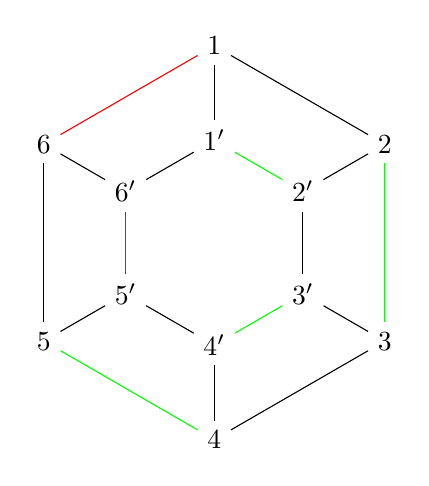
\begin{tikzpicture}
		\foreach \phi in {1,...,6}{
		\node (\phi) at (150 - 360/6 * \phi:1.3cm) {$\phi'$};
		\node (\phi') at (150 - 360/6 * \phi:2.5cm) {$\phi$};
      	};
      	\draw (1) edge[green] (2);
		\draw (2) edge (3);
		\draw (3) edge[green] (4);
		\draw (4) edge (5);
		\draw (5) edge[red] (6);
		\draw (6) edge (1);

		\draw (1') edge (2');
		\draw (2') edge[green] (3');
		\draw (3') edge (4');
		\draw (4') edge[green] (5');
		\draw (5') edge (6');
		\draw (6') edge[red] (1');

		\draw (1) edge (1');
		\draw (2) edge (2');
		\draw (3) edge (3');
		\draw (4) edge (4');
		\draw (5) edge (5');
		\draw (6) edge (6');
	\end{tikzpicture}
	}
	\end{subfloat}
	\hspace{100pt}
	\begin{subfloat}[The minimum forcing number of $P_4 \times K_2$ is $1$.] {
	\centering
	\begin{tikzpicture}
		\foreach \phi in {1,...,4}{
		\node (\phi') at (-1.5,1.5*\phi) {$\phi'$};
		\node (\phi) at (1.5,1.5*\phi) {$\phi$};		
      	};
		\draw (1) edge (2);
		\draw (2) edge[green] (3);
		\draw (3) edge (4);

		\draw (1) edge[green] (1');
		\draw (2) edge (2');
		\draw (3) edge (3');
		\draw (4) edge[green] (4');

		\draw (1') edge (2');
		\draw (2') edge[red] (3');
		\draw (3') edge (4');
	\end{tikzpicture}
	}
	\end{subfloat}
	\caption{The coloured edges form a matching with the red edges being a forcing set.}
	\end{figure}
	% The bipartite adjacency matrix of $P_4$ is
	% \[
	% \begin{pmatrix}
	% 	1 & 0 \\ 1 & 1	
	% \end{pmatrix}.
	% \]
	% In particular, if we weight the nonzero entries of this matrix as $a,b,c$ to get $W$ and the nonzero entries of the transpose as $d,e,f$ to get $W^{-1}$, we have
	% \[ WW^{-1} = \begin{pmatrix} a & 0 \\ b & c \end{pmatrix} \begin{pmatrix} d & e \\ 0 & f \end{pmatrix} = \begin{pmatrix} ad & ae \\ bd & be+cf \end{pmatrix}. \]

	If the forcing number of a matching is $k$, there exists an induced subgraph on $2(n-k)$ vertices with a unique perfect matching. The converse of this need not be true, since we also require that the subgraph on the remaining $2k$ vertices has a perfect matching. For example, the $2 \times n$ grid graph has an induced subgraph on $2n-2$ vertices with a unique perfect matching.

	\begin{figure}[H]
		\centering
		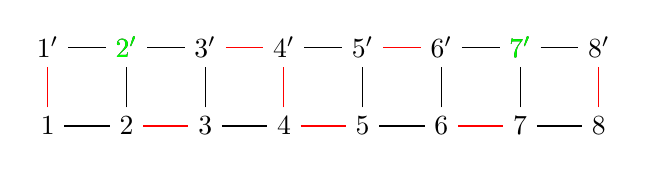
\begin{tikzpicture}
		\foreach \phi in {1,...,8}{
		\node (\phi') at (-5+\phi,0.5) {$\phi'$};
		\node (\phi) at (-5+\phi,-0.5) {$\phi$};		
      	};
      	\node (2') at (-5+2,0.5) {\textcolor{green}{$2'$}};
      	\node (7') at (-5+7,0.5) {\textcolor{green}{$7'$}};
		\draw (1) edge (2);
		\draw (2) edge[red] (3);
		\draw (3) edge (4);
		\draw (4) edge[red] (5);
		\draw (5) edge (6);
		\draw (6) edge[red] (7);
		\draw (7) edge (8);

		\draw (1) edge[red] (1');
		\draw (2) edge (2');
		\draw (3) edge (3');
		\draw (4) edge[red] (4');
		\draw (5) edge (5');
		\draw (6) edge (6');
		\draw (7) edge (7');
		\draw (8) edge[red] (8');

		\draw (1') edge (2');
		\draw (2') edge (3');
		\draw (3') edge[red] (4');
		\draw (4') edge (5');
		\draw (5') edge[red] (6');
		\draw (6') edge (7');
		\draw (7') edge (8');
	\end{tikzpicture}
	\caption{The subgraph on $2n-2$ vertices has a unique perfect matching but the minimum forcing number is $>1$.} 
	\end{figure}

	A \emph{conformal subgraph} is a subgraph such that the subgraph obtained by removing its vertices has a perfect matching. Therefore, if the forcing number of a matching is $k$, there exists an induced conformal subgraph on $2(n-k)$ vertices with a unique perfect matching.

	\begin{question}
		Then, which graphs are such that if their minimum forcing number is $k$, there exists a largest induced subgraph with a unique perfect matching of size $2k$? That is, when does there exist a largest induced subgraph with a unique perfect matching that is also conformal?
	\end{question}

	\begin{question}
		When is the order of the largest induced subgraph with a unique perfect matching equal to twice the min-rank of the bipartite adjacency matrix?
	\end{question}

	Let $G(A,B)$ be a bipartite graph over $2n$ vertices. For a prism $G \times K_2$, the minimum forcing number is at most $n$, for example by matching corresponding vertices in $A$ between the two copies of $G$. If we find a matrix $W$ that has the same non-zero pattern as $A$ such that $W^{-1}$ has the same nonzero pattern as $A^\top$, then the largest induced subgraph with a unique perfect matching has order $2n$, which implies that the minimum forcing number is $n$. A necessary condition for such a $W$ to exist is that no two rows of $A$ have exactly $1$ column in which both rows are $1$. That is, no two vertices in $G$ have exactly one common neighbour.

	\begin{question}
		Is the above necessary condition sufficient? That is, if we have a $0,1$-matrix $A$ such that no two rows have exactly one coordinate where both are $1$, then does there exist a matrix $W$ with the same nonzero pattern as $A$ such that $W^{-1}$ has the same nonzero pattern as $A^\top$? If yes, can we ensure that $W^{-1} = \lambda W^\top$ for some scalar $\lambda$?
	\end{question}

	For example, in the complete bipartite graph $K_{n,n}$ which has bipartite adjacency matrix equal to $J$ (the all $1$s matrix), an example of such a matrix $W$ (for $n=3$, say) is just
	\[
	\begin{pmatrix}
		1 & 1 & 1 \\ 1 & \omega & \omega^2 \\ 1 & \omega^2 & \omega
	\end{pmatrix},
	\]
	where $\omega = e^{2\pi\iota/3}$.\\
	Another example is $K_{n,n}$ with a perfect matching removed (for $n > 3$). For $n=4$, over $\F_2$, the resulting bipartite adjacency matrix is its own inverse. In general, we can take the matrix itself over $\F_p$ for $p$ any prime dividing $n-2$.\\
	
	What happens if we take any bipartite graph $G'$, and then modify it to a graph $G$ by duplicating all the vertices and adding edges $uv'$ if $uv$ is an edge, where $v'$ is the copy of $v$? The bipartite adjacency matrix of this graph is symmetric on taking an appropriate ordering of the vertices. \\

	This question arises from the study of \emph{Hadamard matrices}, which are $n \times n$ $\pm 1$-matrices $H$ such that $HH^\top = n \Id$. There is a famous conjecture stating that such an $H$ exists for $n \equiv 0 \pmod{4}$. There is an easy construction for $n = 2^k$, by taking $H_1 = \begin{pmatrix} 1 \end{pmatrix}$ and
	\[
	H_{2^k} = 
	\begin{pmatrix}
		H_{2^{k-1}} & H_{2^{k-1}} \\ H_{2^{k-1}} & -H_{2^{k-1}}
	\end{pmatrix}.
	\]
	An even more general notion is that of \emph{weighing matrices} $W$, where we allow the entries to be in $\{0,\pm 1\}$ instead of just $\pm 1$ like in Hadamard matrices, and we are interested in having $WW^\top = w \Id$ for some integer $w$. That is, any row has exactly $w$ nonzero entries, and any two rows are orthogonal to each other.

\clearpage